Here is a Gantt chart showing the timeline for my MMath independent project:


\begin{figure}[h] % 'h' means place it here
    \centering
    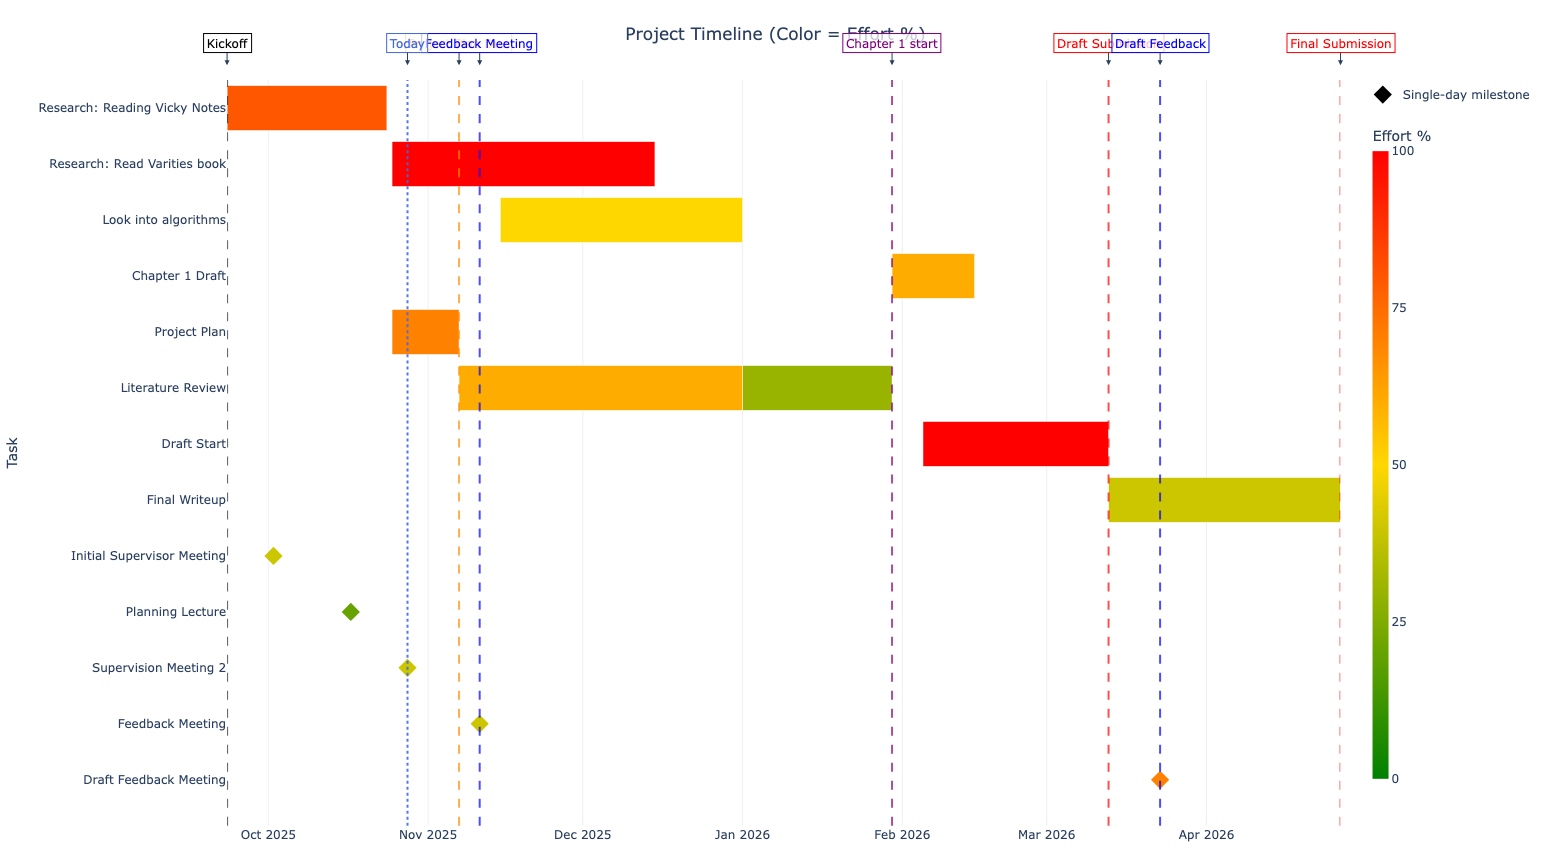
\includegraphics[width=1.2\textwidth]{newplot(3)} % image file name without extension
    \caption{Gantt chart showing the timeline for the MMath independent project.}
    \label{fig:gantt_chart}
\end{figure}

% Make a box with a URL link to interactive Gantt chart
%\begin{center}
%	\fbox{\parbox{0.9\textwidth}{
%		For an interactive version of this Gantt chart, please visit: \\
%		\centering
%		\url{https://www-users.york.ac.uk/~ag1884/}
%	}}
%\end{center}

\begin{center}
\begin{tikzpicture}[every node/.style={align=center}]
  % ---- parameters you might tweak ----
  \def\arrowoffset{5mm}       % how far arrows start from the box
  \def\arrowlen{2.2mm}        % arrowhead size
  \def\poslist{0.12,0.32,0.52,0.72,0.88} % positions along each side (0..1)

  % ---- the box ----
  \node[draw, very thick, rounded corners=1pt,
        inner sep=8pt, text width=.78\linewidth] (box)
  {For an interactive version of this Gantt chart, please visit:\\
   \textbf{\url{https://www-users.york.ac.uk/~ag1884/}}};

  % ---- arrows on TOP (pointing down) ----
  \foreach \t in \poslist {
    \draw[-{Latex[length=\arrowlen]}, thick]
      ($ (box.north west)!\t!(box.north east) + (0,\arrowoffset) $)
      -- ($ (box.north west)!\t!(box.north east) $);
  }

  % ---- arrows on BOTTOM (pointing up) ----
  \foreach \t in \poslist {
    \draw[-{Latex[length=\arrowlen]}, thick]
      ($ (box.south west)!\t!(box.south east) + (0,-\arrowoffset) $)
      -- ($ (box.south west)!\t!(box.south east) $);
  }

  % ---- arrows on LEFT (pointing right) ----
  \foreach \t in \poslist {
    \draw[-{Latex[length=\arrowlen]}, thick]
      ($ (box.south west)!\t!(box.north west) + (-\arrowoffset,0) $)
      -- ($ (box.south west)!\t!(box.north west) $);
  }

  % ---- arrows on RIGHT (pointing left) ----
  \foreach \t in \poslist {
    \draw[-{Latex[length=\arrowlen]}, thick]
      ($ (box.south east)!\t!(box.north east) + (\arrowoffset,0) $)
      -- ($ (box.south east)!\t!(box.north east) $);
  }
\end{tikzpicture}
\end{center}

\section*{Written Commentary of plan}
The Gantt chart in Figure~\ref{fig:gantt_chart} outlines the timeline for my MMath independent project. The project is structured into several key phases, each with specific tasks and milestones.

{\bf Note:} The weeks mentioned correspond to the academic calendar of the University of York for the 2025-2026 academic year. Also some tasks overlap to allow for flexibility and ensure that progress can be made even if certain tasks take longer than expected. The dates are also speculative and may change based on my progress and any unforeseen circumstances.

\begin{itemize}
	\item \textbf{Initial Research (Weeks 1-5):}  During this part, I focused on reading the lecure notes of my supervisor Prof Victoria Gould and relevant material from book "Automata and Languages" by John M. Howie. This helped me understand the basics of DFA's and syntactic monoids
	\item \textbf{Project Plan (Weeks 5-6)}: I started working on my project plan. This also relied on me consulting additonal literaturein tandem.
	\item \textbf{Study on Varieties (Weeks 6-12):} This phase involves a deep dive into the theoretical and computational aspects of pseudovarieties of finite monoids and their applications in formal languages and automata theory. I will study Eilenberg's correspondence and related concepts. Most of this material is covered in the book "Varieties of Formal Languages" by Jean-Éric Pin and his lecture notes available online.
	\begin{itemize}
		\item October 25-December 15: Read through relevant chapters of Jean-Éric Pin's book and understand the theoretical concepts.
		\item November 15-January 1: Look into algorithms used to generate syntactic monoids of regular languages and test membership in pseudovarieties.
		\item November 15-January 30th: I will also read alternative literature and look up other references.
		
		\textbf{Note:} January 1-30th is reading week and exam period so I will not be doing much work on the project during this time.
	\end{itemize}
	\item January 30-February 15: Start the draft, I will try and write up the first few chapters and theoretical background during this time.
		\item February 5-March 13: Start and finish draft before deadline. I will also write code to compute syntactic monoids of small DFAs using GAP. If time permits, I will also try and implement algorithms to test membership in certain pseudovarieties of finite monoids.
		\item March 13-April 27: Final revisions and submission. I will review the entire document, make necessary revisions, and prepare the final version for submission by the deadline. I will start the final version before the draft feedback to ensure I have enough time to make revisions based on the feedback received.
\end{itemize}